\section*{Representation \& Description}

Two ways of representing region:

\begin{itemize}
  \item \textbf{Representation:} in terms of its external
    characteristics (its boundary):
    focus on shape characteristics
  \item \textbf{Description:} in terms of its internal
    characteristics (its region): focus
    on regional properties, e.g., color, texture
\end{itemize}

\subsection*{Sensitivity}

Features selected as descriptors should be as \textbf{insensitive} as
possible to: (i) size, (ii) translation and (iii) rotation

\subsection*{Representation}

\begin{itemize}
  \item Segmentation techniques yield raw data in the form of:
    (i) pixels along a boundary or (ii) pixels contained in a region
  \item These data sometimes are used directly to obtain \textbf{descriptors}
  \item Useful data (descriptors) are extracted from the raw data
    to reduce the amount of data to be processed
\end{itemize}

\subsubsection*{Chain Codes}

Based on the \textbf{4- or 8-connectivity of pixels}, a chain code is a
sequence of directions that describes the boundary of a region.

Usually unacceptable because:

\begin{itemize}
  \item \textbf{Length:} The resulting chain of codes tends to be quite long
  \item \textbf{Sensitivity to Noise:} Small disturbances along the
    boundary due to (i) noise or (ii) imperfect segmentation cause
    changes in the code that may not be related to the shape of the boundary
\end{itemize}

\textbf{Solution:} Resample the boundary by selecting larger grid spacing.
Different grid can generate different chain codes.

\begin{figure}[H]
  \centering
  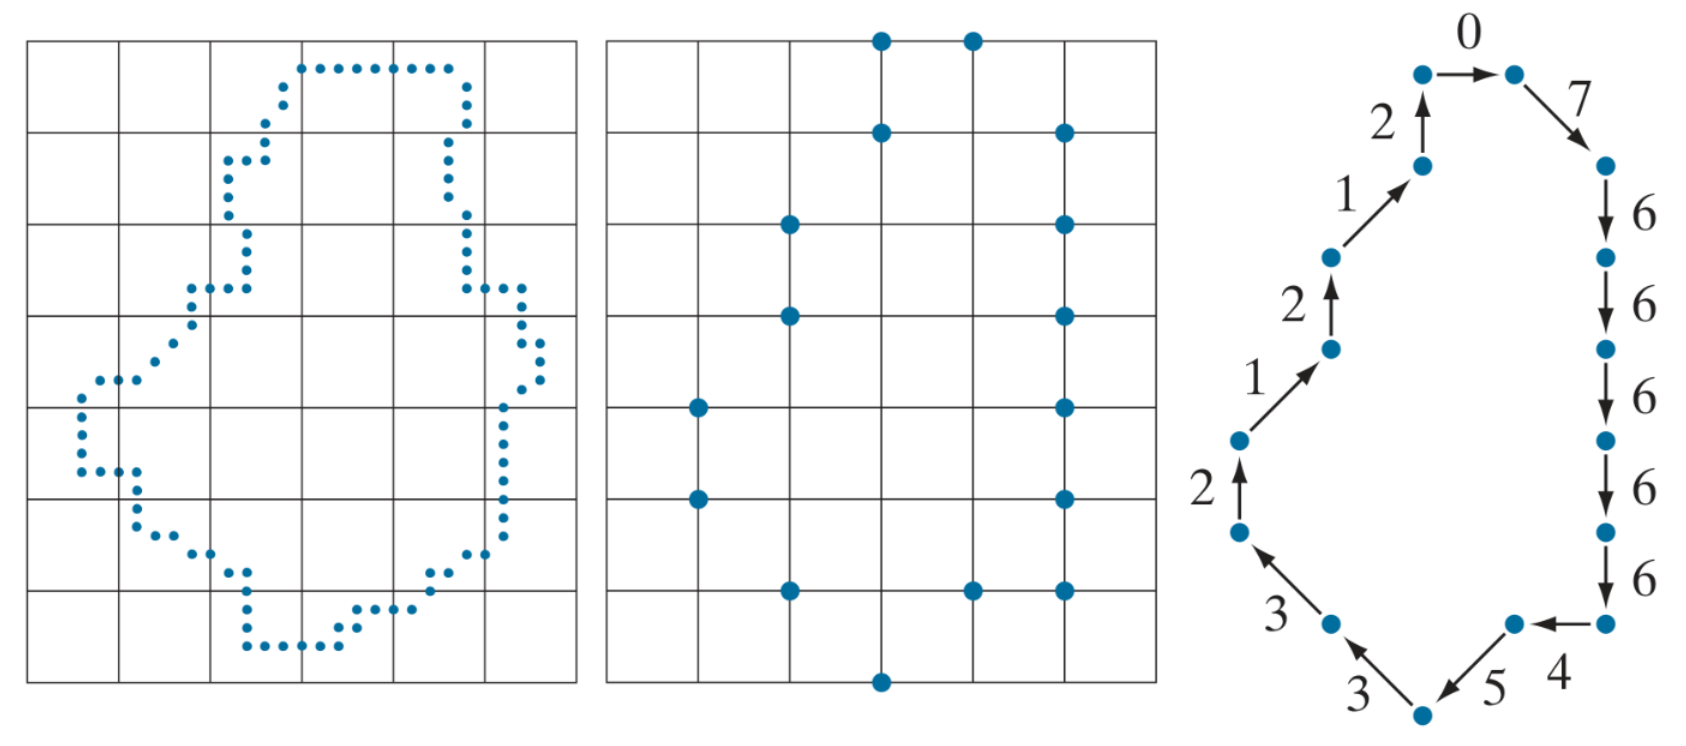
\includegraphics[width=\linewidth]{images/chain_code.png}
  \caption{Resampling to a larger grid, then using 8-neighbor chain code}
\end{figure}

\subsubsection*{Polygonal Approximation}

\begin{itemize}
  \item Boundary can be approximated with arbitrary accuracy by a polygon
  \item Try to capture the \enquote{essence} of the boundary shape
    with the fewest possible polygonal segments
  \item \textbf{Minimum Perimeter Polygon (MPP):} One of the most efficient ways
  \item Not trivial and time consuming
\end{itemize}

\begin{figure}[H]
  \centering
  \includegraphics[width=\linewidth]{images/polygonal_approximation.png}
  \caption{Minimum Perimeter Polygon (MPP) obtained by allowing the
  boundary to shrink to the grid}
\end{figure}

\subsubsection*{Splitting Techniques}

\begin{enumerate}

  \item Find the major axis
  \item Find minor axes which is perpendicular to major axis and has
    distance greater than a threshold
  \item Repeat until we can't split anymore
\end{enumerate}

\begin{figure}[H]
  \centering
  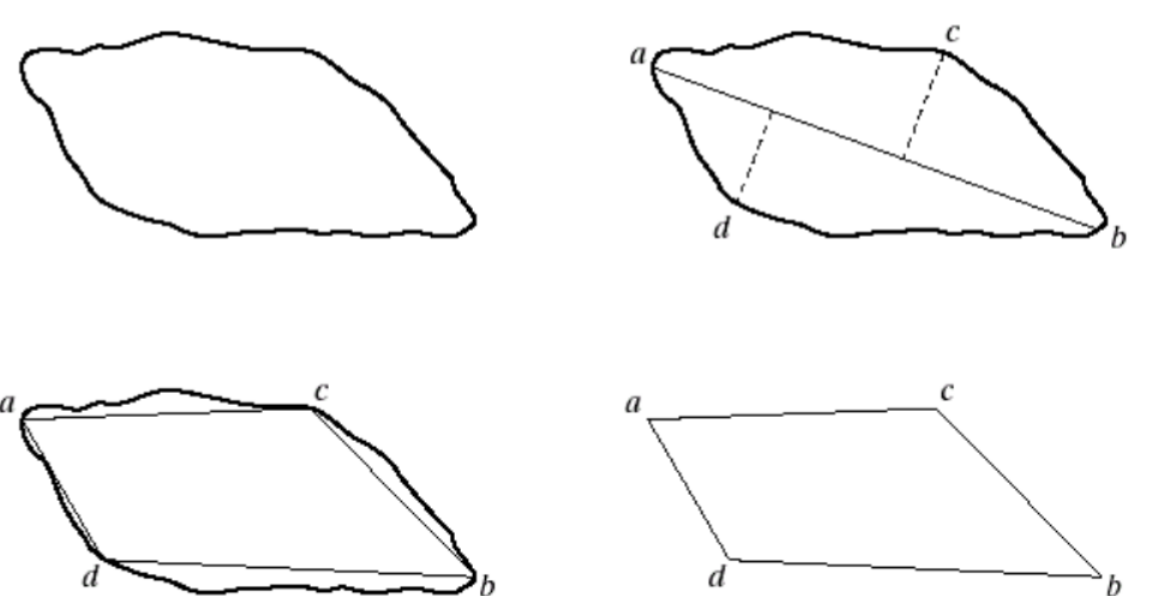
\includegraphics[width=\linewidth]{images/splitting.png}
  \caption{Dividing the boundary based on extreme points, then
  joining them using segments}
\end{figure}

\subsubsection*{Signatures}

\textbf{Signature} is a 1-D functional representation of a 2-D boundary.

\begin{itemize}
  \item Simplest technique: plot the distance of the boundary from
    the centroid ($r$) to the boundary as a function of angle ($\theta$)
  \item Samples are taken at regular intervals of angle $\theta$
\end{itemize}

\begin{figure}[H]
  \centering
  \includegraphics[width=\linewidth]{images/signatures.png}
  \caption{Signatures of circular vs square boundaries}
\end{figure}

\begin{figure}[H]
  \centering
  \includegraphics[width=\linewidth]{images/binary_regions_signatures.png}
  \caption{Signatures of some irregular binary regions}
\end{figure}

\subsubsection*{Convex Hull/Boundary Segments}

A convex hull $H$ of an arbitrary set $S$ is the \textbf{smallest
convex set} containing $S$.

The set difference $H - S$ is called the \textbf{convex deficiency} $D$ of $S$.

\begin{figure}[H]
  \centering
  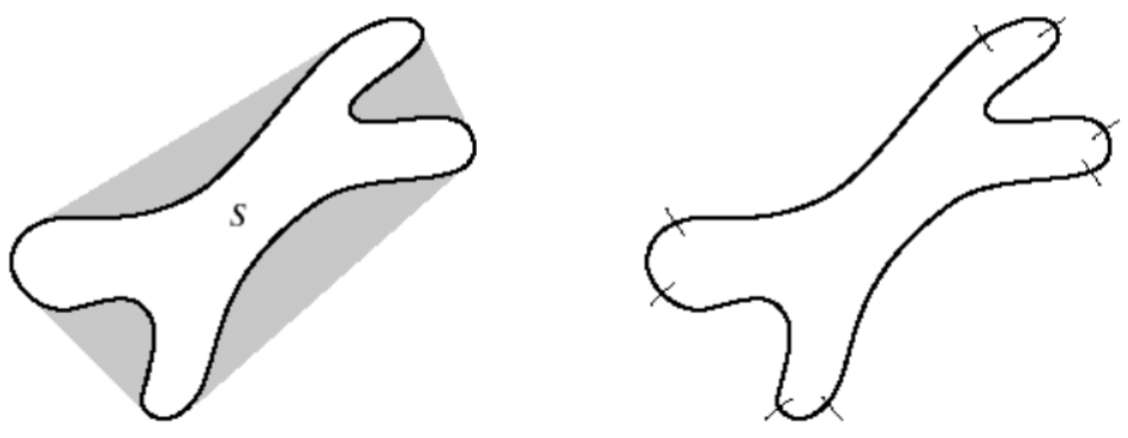
\includegraphics[width=\linewidth]{images/convex_hull_boundary_segments.png}
  \caption{Convex hull of a region (left), partitioned boundary (right)}
\end{figure}

\subsubsection*{Skeletonization}

A \textbf{skeleton} of a region is a thin version of the region. Also
known as \textbf{medial axis}.

\begin{figure}[H]
  \centering
  \includegraphics[width=\linewidth]{images/skeletonization.png}
  \caption{Process of skeletonizing a region; (i) the dashed lines
    represent the skeleton (ii) the circles are \enquote{maximum
    disks}, the largest disks centered at any point inside the region
  and contained in the region.}
\end{figure}

\begin{figure}[H]
  \centering
  \includegraphics[width=\linewidth]{images/skeleton_handwritten.png}
  \caption{Skeleton of binarized handwritten characters}
\end{figure}

\subsection*{Boundary Descriptors}

\subsubsection*{Length of a Boundary}

The \textbf{number of pixels along a boundary} gives a rough
approximation of its length

\subsubsection*{Diameter}

\begin{equation*}
  \text{Diam}(B) = \max_{i, j}[D(p_i, p_j)]
\end{equation*}

$D \rightarrow$ distance measure, $p_i, p_j \rightarrow$ points on boundary $B$.

\subsubsection*{Eccentricity}

Ratio of the \textbf{major axis} to the \textbf{minor axis}:

\begin{itemize}
  \item \textbf{Major axis:} Line connecting the two extreme points
    that comprise the diameter
  \item \textbf{Minor axis:} Line perpendicular to the major axis
    that passes through the centroid of the region
\end{itemize}

\subsection*{Regional Descriptors}

\subsubsection*{Simple Descriptors}

\begin{itemize}
  \item \textbf{Area:} The number of pixels in the region
  \item \textbf{Perimeter:} Length of the boundary
  \item \textbf{Compactness:} $\text{Comp} =
    \frac{\text{Perimeter}^2}{\text{Area}}$

\end{itemize}

\subsubsection*{Topological Descriptors}

\begin{itemize}
  \item \textbf{Euler number:} $\chi = C - H$, where $C$ is the
    number of connected components and $H$ is the number of holes
\end{itemize}

\begin{figure}[H]
  \centering
  \includegraphics[width=\linewidth]{images/euler_numbers.png}
  \caption{Two regions with Euler number 0 and -1 respectively}
\end{figure}
